\documentclass[tikz,border=8pt]{standalone}
\usepackage{tikz}
\usepackage{amsmath,amssymb}
\usetikzlibrary{shapes.geometric, arrows.meta, positioning, fit, backgrounds, calc}

\definecolor{cefnblue}{HTML}{2E86AB}
\definecolor{evo2mag}{HTML}{A23B72}
\definecolor{amorange}{HTML}{F18F01}
\definecolor{priororange}{HTML}{E67E22}
\definecolor{evidencepurple}{HTML}{9B59B6}
\definecolor{pathred}{HTML}{C73E1D}
\definecolor{benignblue}{HTML}{2E86AB}
\definecolor{vusgray}{HTML}{8D99AE}
\definecolor{boxbg}{HTML}{F8F9FA}
\definecolor{arrowgray}{HTML}{7F8C8D}
\definecolor{dark}{HTML}{2B2D42}

\begin{document}
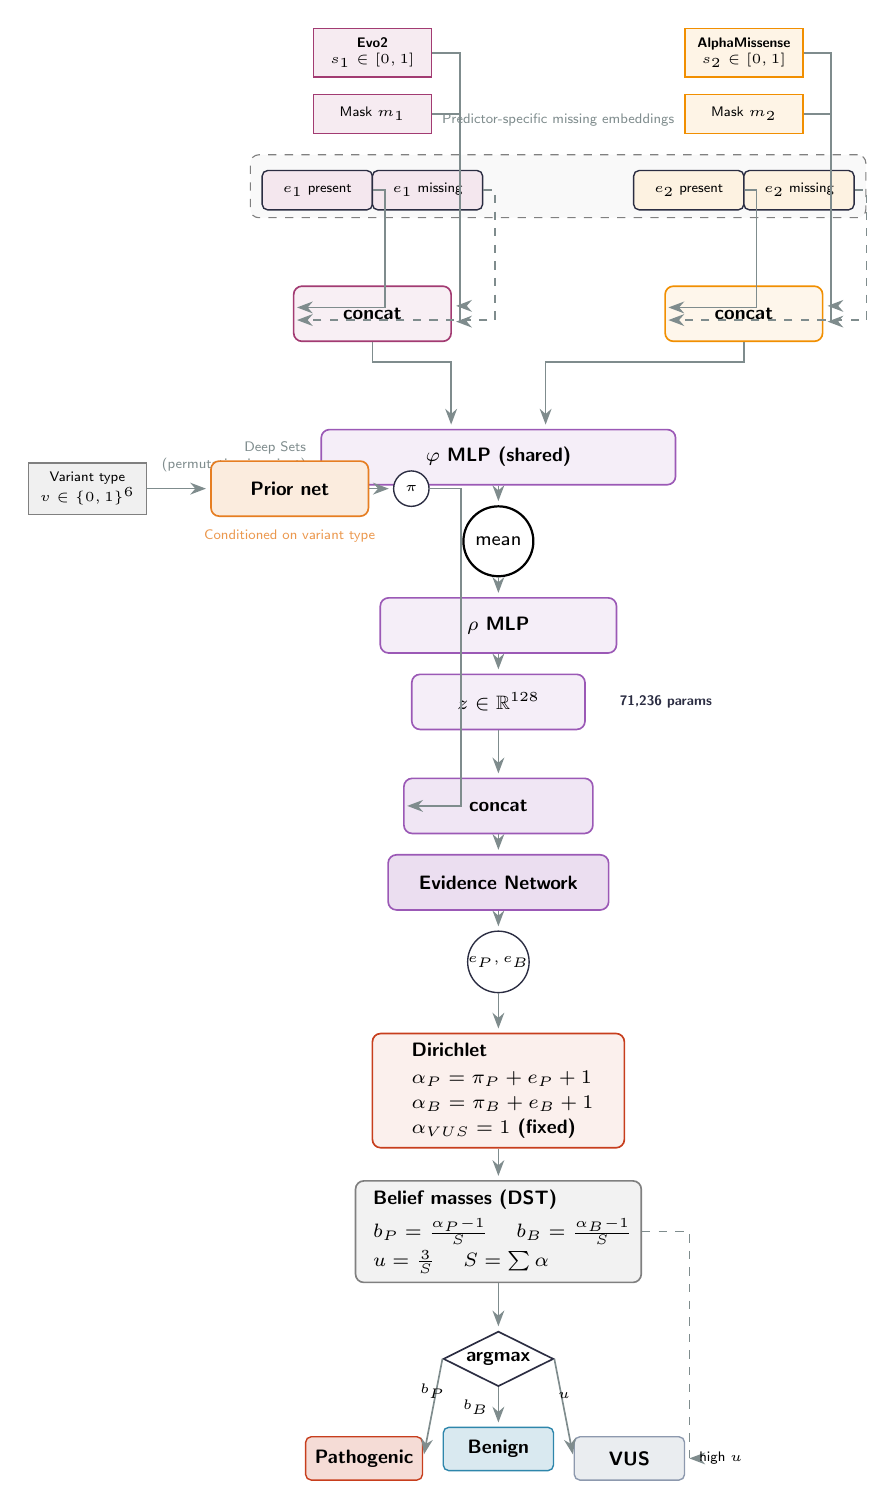
\begin{tikzpicture}[
    font=\sffamily\scriptsize,
    >=Stealth,
    thick,
    input/.style={rectangle, draw=dark, fill=white, minimum width=1.5cm, minimum height=0.5cm,
                  align=center, line width=0.5pt, font=\sffamily\tiny},
    embed/.style={rectangle, draw=dark, fill=#1!12, minimum width=1.4cm, minimum height=0.5cm,
                  align=center, rounded corners=2pt, line width=0.5pt, font=\sffamily\tiny},
    network/.style={rectangle, draw=dark, fill=boxbg, minimum width=2.0cm, minimum height=0.7cm,
                      align=center, font=\sffamily\scriptsize\bfseries, rounded corners=3pt, line width=0.6pt},
    param/.style={circle, draw=dark, fill=white, minimum size=0.45cm, inner sep=0pt, line width=0.5pt, font=\sffamily\tiny},
    decision/.style={diamond, draw=dark, fill=white, aspect=2, minimum width=1.4cm, minimum height=0.7cm,
                     align=center, font=\sffamily\scriptsize\bfseries, inner sep=0pt, line width=0.6pt},
    output/.style={rectangle, draw=dark, fill=#1!18, minimum width=1.4cm, minimum height=0.55cm,
                   align=center, font=\sffamily\scriptsize\bfseries, rounded corners=2pt, line width=0.5pt},
    arrow/.style={->, line width=0.6pt, draw=arrowgray, shorten >=1.5pt},
    dasharrow/.style={->, line width=0.6pt, draw=arrowgray, dashed, shorten >=1.5pt},
    annot/.style={font=\sffamily\tiny, text=arrowgray}
]

% ==================================================================
% ROW 1: INPUTS (side by side)
% ==================================================================
\node[input, fill=evo2mag!10, draw=evo2mag] (evo2s) 
    {\textbf{Evo2}\\$s_1 \in [0,1]$};
\node[input, fill=evo2mag!10, draw=evo2mag, below=0.2cm of evo2s] (evo2m) 
    {Mask $m_1$};

\node[embed=evo2mag, below=0.45cm of evo2m, xshift=-0.7cm] (evo2e) 
    {$e_1$ present};
\node[embed=evo2mag, below=0.45cm of evo2m, xshift=+0.7cm] (evo2miss) 
    {$e_1$ missing};

\node[network, fill=evo2mag!8, draw=evo2mag, below=0.95cm of evo2e, xshift=0.7cm, minimum width=2.0cm] (evo2cat) 
    {concat};

\coordinate (e2in1) at ([yshift=0.10cm, xshift=0.15cm]evo2cat.east);
\coordinate (e2in2) at ([yshift=-0.10cm, xshift=0.15cm]evo2cat.east);
\draw[arrow] (evo2s.east) -- ++(0.35,0) |- (e2in1) -- ([yshift=0.10cm]evo2cat.east);
\draw[arrow] (evo2m.east) -- ++(0.35,0) |- (e2in2) -- ([yshift=-0.10cm]evo2cat.east);
\draw[arrow] (evo2e.east) -- ++(0.15,0) |- ([yshift=0.08cm]evo2cat.west);
\draw[dasharrow] (evo2miss.east) -- ++(0.15,0) |- ([yshift=-0.08cm]evo2cat.west);

% --- AM branch (right) ---
\node[input, fill=amorange!10, draw=amorange, right=3.2cm of evo2s] (ams) 
    {\textbf{AlphaMissense}\\$s_2 \in [0,1]$};
\node[input, fill=amorange!10, draw=amorange, below=0.2cm of ams] (amm) 
    {Mask $m_2$};

\node[embed=amorange, below=0.45cm of amm, xshift=-0.7cm] (ame) 
    {$e_2$ present};
\node[embed=amorange, below=0.45cm of amm, xshift=+0.7cm] (ammiss) 
    {$e_2$ missing};

\node[network, fill=amorange!8, draw=amorange, below=0.95cm of ame, xshift=0.7cm, minimum width=2.0cm] (amcat) 
    {concat};

\coordinate (amin1) at ([yshift=0.10cm, xshift=0.15cm]amcat.east);
\coordinate (amin2) at ([yshift=-0.10cm, xshift=0.15cm]amcat.east);
\draw[arrow] (ams.east) -- ++(0.35,0) |- (amin1) -- ([yshift=0.10cm]amcat.east);
\draw[arrow] (amm.east) -- ++(0.35,0) |- (amin2) -- ([yshift=-0.10cm]amcat.east);
\draw[arrow] (ame.east) -- ++(0.15,0) |- ([yshift=0.08cm]amcat.west);
\draw[dasharrow] (ammiss.east) -- ++(0.15,0) |- ([yshift=-0.08cm]amcat.west);

% Background box around embedding layer only, label above
\scoped[on background layer]{
    \node[fit=(evo2e)(evo2miss)(ame)(ammiss), draw=gray, dashed, fill=gray!5,
          inner sep=4pt, rounded corners=3pt, yshift=0.05cm] (embed_region) {};
}
\node[annot, above=0.22cm of embed_region.north, anchor=south] {Predictor‑specific missing embeddings};

% ==================================================================
% ROW 2: DEEP SETS (centered below)
% ==================================================================
\node[network, fill=evidencepurple!10, draw=evidencepurple, below=1.1cm of evo2cat, xshift=1.6cm, minimum width=4.5cm] (deepset_phi) 
    {$\varphi$ MLP (shared)};

\node[draw, circle, fill=white, minimum size=0.55cm, below=0.25cm of deepset_phi] (meanpool) {mean};
\node[network, fill=evidencepurple!10, draw=evidencepurple, below=0.25cm of meanpool, minimum width=3.0cm] (deepset_rho) 
    {$\rho$ MLP};
\node[network, fill=evidencepurple!10, draw=evidencepurple, below=0.25cm of deepset_rho, minimum width=2.2cm] (deepset_out) 
    {$z \in \mathbb{R}^{128}$};

\draw[arrow] (evo2cat.south) -- ++(0,-0.25) -| ([xshift=-0.6cm]deepset_phi.north);
\draw[arrow] (amcat.south) -- ++(0,-0.25) -| ([xshift=0.6cm]deepset_phi.north);
\draw[arrow] (deepset_phi.south) -- (meanpool.north);
\draw[arrow] (meanpool.south) -- (deepset_rho.north);
\draw[arrow] (deepset_rho.south) -- (deepset_out.north);

\node[annot, left=0.05cm of deepset_phi.west, anchor=east, align=right] 
    {Deep Sets\\(permutation‑invariant)};

% ==================================================================
% ROW 3: PRIOR + EVIDENCE (side by side)
% ==================================================================
\node[input, fill=gray!12, draw=gray, left=2.2cm of deepset_phi.west, yshift=-0.4cm] (vartype) 
    {Variant type\\$v \in \{0,1\}^6$};
\node[network, fill=priororange!15, draw=priororange, right=0.8cm of vartype] (priornet) 
    {Prior net};
\node[param, right=0.3cm of priornet] (prior_alpha) 
    {$\pi$};

\draw[arrow] (vartype.east) -- (priornet.west);
\draw[arrow] (priornet.east) -- (prior_alpha.west);
\node[annot, below=0.03cm of priornet.south, text=priororange!80] {Conditioned on variant type};

% Evidence
\node[network, fill=evidencepurple!15, draw=evidencepurple, below=0.6cm of deepset_out, minimum width=2.4cm] (concat_evidence) 
    {concat};
\draw[arrow] (deepset_out.south) -- ++(0,-0.15) -| (concat_evidence.north);
\draw[arrow] (prior_alpha.east) -- ++(0.4,0) |- (concat_evidence.west);

\node[network, fill=evidencepurple!20, draw=evidencepurple, below=0.25cm of concat_evidence, minimum width=2.8cm] (evidencenet) 
    {Evidence Network};
\node[param, below=0.25cm of evidencenet] (evidence_e) 
    {$e_P, e_B$};
\draw[arrow] (concat_evidence.south) -- (evidencenet.north);
\draw[arrow] (evidencenet.south) -- (evidence_e.north);

% ==================================================================
% ROW 4: DIRICHLET + BELIEF (side by side, compact)
% ==================================================================
\node[network, fill=pathred!8, draw=pathred, below=0.5cm of evidence_e, minimum width=3.2cm, minimum height=1.1cm, align=left] (dirichlet) 
    {\hspace{3pt}\textbf{Dirichlet}\\[2pt]
     \hspace{3pt}$\alpha_P = \pi_P + e_P + 1$\\[1pt]
     \hspace{3pt}$\alpha_B = \pi_B + e_B + 1$\\[1pt]
     \hspace{3pt}$\alpha_{VUS} = 1$ \textbf{(fixed)}};

\draw[arrow] (evidence_e.south) -- (dirichlet.north);

\node[network, fill=gray!10, draw=gray, below=0.4cm of dirichlet, minimum width=3.6cm, minimum height=1.0cm, align=left] (beliefs) 
    {\hspace{3pt}\textbf{Belief masses (DST)}\\[2pt]
     \hspace{3pt}$b_P = \frac{\alpha_P-1}{S}$ \quad
     $b_B = \frac{\alpha_B-1}{S}$\\[1pt]
     \hspace{3pt}$u = \frac{3}{S}$ \quad
     $S = \sum\alpha$};

\draw[arrow] (dirichlet.south) -- (beliefs.north);

% ==================================================================
% ROW 5: DECISION + OUTPUTS (compact)
% ==================================================================
\node[decision, below=0.6cm of beliefs] (decision) 
    {\textbf{argmax}};
\draw[arrow] (beliefs.south) -- (decision.north);

\node[output=pathred, draw=pathred, below left=0.8cm and 0.6cm of decision] (outP) 
    {Pathogenic};
\node[output=benignblue, draw=benignblue, below=0.5cm of decision] (outB) 
    {Benign};
\node[output=vusgray, draw=vusgray, below right=0.8cm and 0.6cm of decision] (outV) 
    {VUS};

\draw[arrow] (decision.west) -- (outP.east) node[pos=0.5, above, font=\sffamily\tiny] {$b_P$};
\draw[arrow] (decision.south) -- (outB.north) node[pos=0.5, left, font=\sffamily\tiny] {$b_B$};
\draw[arrow] (decision.east) -- (outV.west) node[pos=0.5, above, font=\sffamily\tiny] {$u$};

\draw[dasharrow] (beliefs.east) -- ++(0.6,0) |- (outV.east) node[pos=0.5, right, font=\sffamily\tiny] {high $u$};

% ==================================================================
% PARAMETER COUNT (moved to not overlap)
% ==================================================================
\node[annot, right=0.3cm of deepset_out.east, text=dark, anchor=west] 
    {\textbf{71,236 params}};

\end{tikzpicture}
\end{document}
